\subsection{Robust KnapSack Problem}
In this problem we'll solve the classic Knapsack problem with an added uncertainty on the volumes of the items

\paragraph*{Finite uncertainty set}
In general for finite sets, the only one that leads to a viable result is the one where the uncertainty budget is 0.

\paragraph*{Ellipsoidal uncertainty set}
We can see that the probability of violation decreases as the uncertainty budget / ellipsiod radius increases. This is expected since the larger the uncertainty set, the more likely it is that the solution is feasible.
\begin{figure}[H]
    \centering
    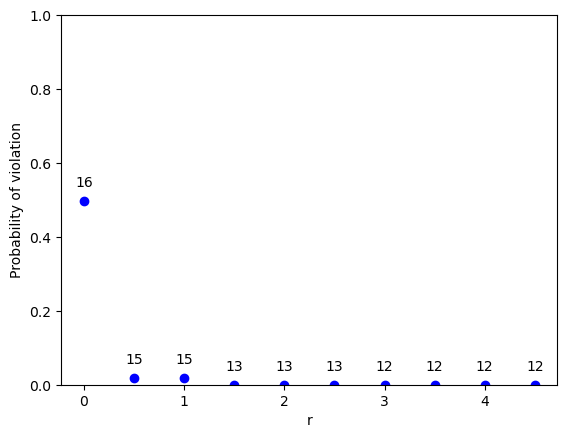
\includegraphics[width=0.5\textwidth]{lab12/imgs/ellips.png}
    \caption{Probability of violation for different uncertainty budgets $r$}
    \label{fig:ellips}
\end{figure}

\subsection{Robust Portfolio Optimization}
In this problem we have a set of fictionary stocks, each one with a different mean and deviation on the return.
We want to robustly maximize the return with a box uncertainty set.

\paragraph*{Box uncertainty set}
The box uncertainty set is defined as a lower and upper bound. For almost all possible boxes, the algorithm always return stock F which is the one with the highest return. The only exception is for negative boxes, where the algorithm return stock H which is the one with the lowest deviation.
\begin{figure}[H]
    \begin{subfigure}{0.5\textwidth}
        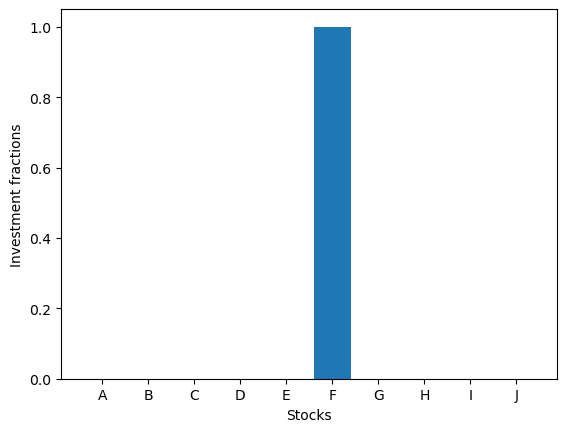
\includegraphics[width=\textwidth]{lab12/imgs/pos_bounds.png}
        \caption{Positive box uncertainty set}
    \end{subfigure}
    \begin{subfigure}{0.5\textwidth}
        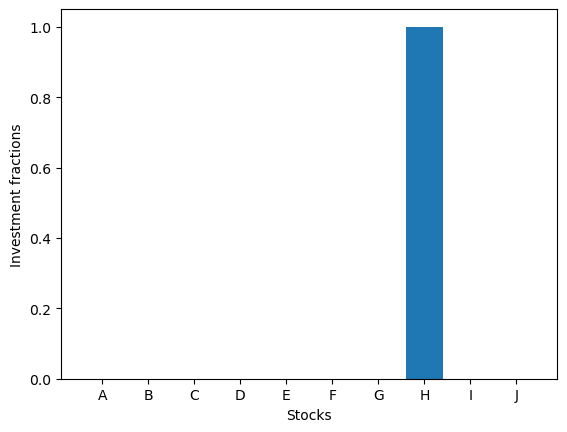
\includegraphics[width=\textwidth]{lab12/imgs/neg_bounds.png}
        \caption{Negative  uncertainty set}
    \end{subfigure}
    \label{fig:box}
\end{figure}

\paragraph*{Norm uncertainty set}
We can see how the return decreases as the upper bound increases. This is expected since the algorithm is trying to maximize the return while keeping the uncertainty low.

\begin{figure}[H]
    \begin{subfigure}{0.5\textwidth}
        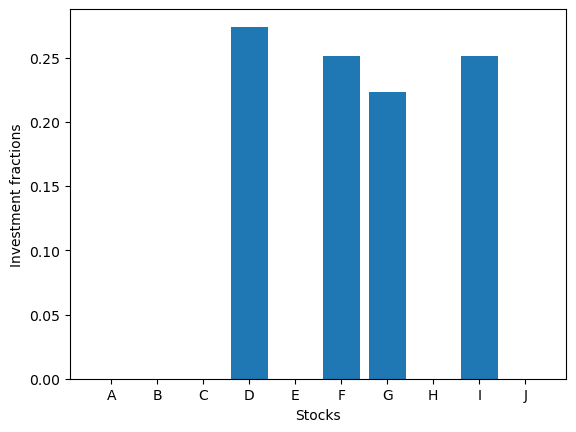
\includegraphics[width=\textwidth]{lab12/imgs/norm_05.png}
        \caption{Upper bound = 0.5}
    \end{subfigure}
    \begin{subfigure}{0.5\textwidth}
        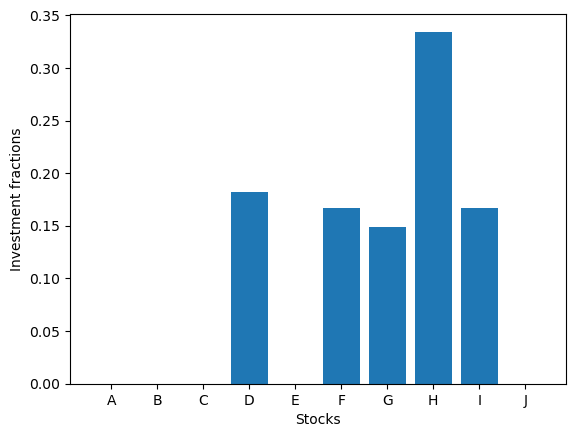
\includegraphics[width=\textwidth]{lab12/imgs/norm_10.png}
        \caption{Upper bound = 1.0}
    \end{subfigure}\\
    \begin{subfigure}{0.5\textwidth}
        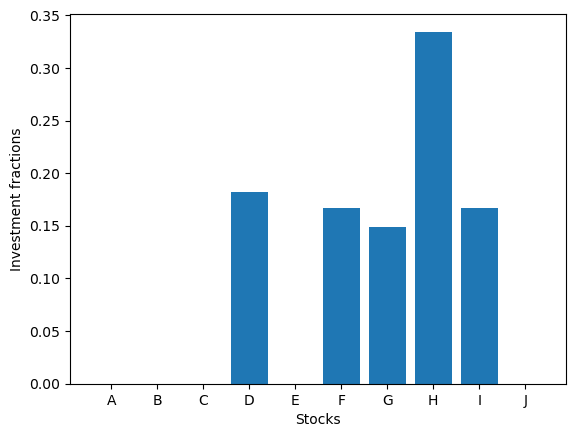
\includegraphics[width=\textwidth]{lab12/imgs/norm_15.png}
        \caption{Upper bound = 1.5}
    \end{subfigure}
    \begin{subfigure}{0.5\textwidth}
        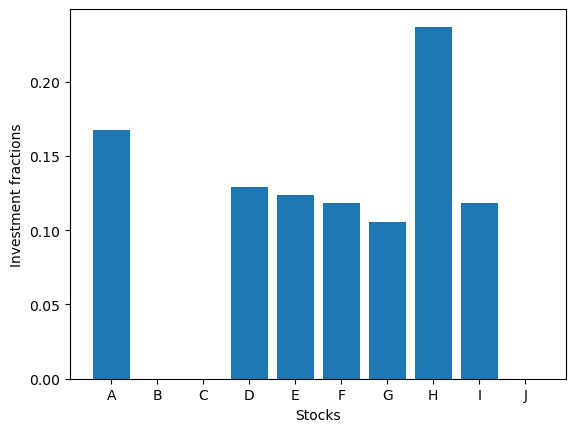
\includegraphics[width=\textwidth]{lab12/imgs/norm_20.png}
        \caption{Upper bound = 2.0}
    \end{subfigure}
    \label{fig:norm}
\end{figure}

\begin{table}[H]
    \centering
    \begin{tabular}{|c|c|}
        Upper bound & Objective value \\ \hline
        0.5         & 1.0196          \\
        1.0         & 0.9963          \\
        1.5         & 0.9763          \\
        2.0         & 0.9602          \\
        \hline
    \end{tabular}
    \caption{Results for different upper bounds}
\end{table}